%\documentclass[handout]{rsuqbeamernew}
\documentclass{rsuqbeamernew}
\def\ANIMATE{0}   %   0/1: Compile animations or not

%%%%%%%%%%%%%%%%%%%%%%%%%%%%%%%%%%%%%%%%%%%%%%%%%%%%%%%%%%%%%%%%%%%%%%%%%%%%%%%%%%%%%%%%%%%%%%%%%%%%%%
%
%
%
\title[HPC Meeting]{Dispatcher Restart}
\subtitle{HPC Meeting}
\institute[Chair of Risk \& Safety] {}
\author[D. Wicaksono]{Damar Wicaksono}

\date[December 03, 2019] {\small December 03, 2019}

% graphics
\graphicspath{{Figures/},{Figures/Christos/}}

\usepackage{bstnotations}
\usepackage[noend]{algpseudocode}
\usepackage{algorithm}
\usepackage{animate}
\usepackage{listings}

\definecolor{matlabComment}{rgb}{0.13,0.55,0.13}
\lstset{language=Matlab,
  basicstyle=\lstbasicfont\upshape\scriptsize,
  keywordstyle=\color{blue},
  numberstyle=\tiny,
  frame=shadowbox,rulesepcolor=\color{gray},
  commentstyle=\lstbasicfont\scriptsize\upshape\bf\color{matlabComment},
  breaklines=false,
  showstringspaces=false,
  morekeywords={uqlab,uq_retrieveSession,uq_create_xyz, 
    uq_createInput,uq_createModel,uq_createAnalysis,
    uq_createDispatcher,uq_set_workflow,UQ_input,
    UQ_model,UQ_analysis,UQ_dispatcher,
    UQ_workflow,UQ, uq_runAnalysis, uq_runAnalysis,
    uq_create_hpc_dispatcher,
    uq_retrieveSession,uq_get_model_response,
    uq_calculateMetamodel, uq_getSample,
    uq_enrichSample,uq_default_input,
    uq_enrichLHS, uq_enrichSobol, uq_enrichHalton, uq_LHSify,
    uq_evalModel, uq_runModel, uq_runAnalysis,
    uq_selectInput,uq_selectAnalysis,uq_selectModel,uq_select_xyz,
    uq_getInput,uq_getAnalysis,uq_getModel,
    uq_setDefaultSampling,uq_GeneralIsopTransform,uq_IsopTransform,
    uq_sampleU,
    uq_NatafTransform, uq_invNatafTransform, uq_MarginalFields,
    uq_print, uq_display
  },
  xleftmargin=0.03\textwidth,
  xrightmargin=0.03\textwidth,
  aboveskip=2mm,
  belowskip=2mm,
  tabsize=1,
  %    linewidth=\textwidth,
  literate={~} {$\sim$}{1}
}

% additional
\newcommand{\card}[1]{\mathrm{card}(#1)}
\DeclareMathOperator*{\argmax}{arg\,max}
\DeclareMathOperator*{\argmin}{arg\,min}

% algorithm abbreviations
\newcommand{\Ntot}{\textsc{Ntot}}
\newcommand{\Ninit}{\textsc{Ninit}}
\newcommand{\M}{\textsc{M}}
\newcommand{\Nneigh}{\textit{NNeighbour}}
\newcommand{\NBound}{\textsc{NBoundaries}}
\newcommand{\NneighThresh}{\textsc{NNeighbourThreshold}}
\newcommand{\Penal}{\textit{Penalization}}
\newcommand{\Pmax}{\textsc{Pmax}}
\newcommand{\NRefine}{\textsc{NRefine}}
\newcommand{\NRefineIter}{\textsc{NEnrIter}}
\newcommand{\Func}[1]{\textsc{model}(#1)}
\newcommand{\Inp}[1]{\textsc{input}(#1)}
\newcommand{\X}{\textit{X}}
\newcommand{\Xcurr}{\textit{Xcurr}}
\newcommand{\Xnew}{\textit{Xnew}}
\newcommand{\Y}{\textit{Y}}
\newcommand{\Ycurr}{\textit{Ycurr}}
\newcommand{\Ynew}{\textit{Ynew}}
\newcommand{\PCEref}{\textit{PCEpar}}
\newcommand{\Dref}{\textit{Dpar}}
\newcommand{\Di}{\textit{Di}}
\newcommand{\Dcand}{\textit{Dcand}}
\newcommand{\Dfirst}{\textit{D1}}
\newcommand{\Dsec}{\textit{D2}}
\newcommand{\Dnew}{\textit{Dchild}}
\newcommand{\Res}{\textit{Resid}}
\newcommand{\Rescurr}{\textit{ResidualCurr}}
\newcommand{\Errors}[1]{\textit{Errors}#1}
\newcommand{\ErrorLoo}{\textit{ErrorLOO}}
\newcommand{\Domain}[1]{\textit{Domains}#1}
\newcommand{\PCEs}[1]{\textit{PCEs}#1}
\newcommand{\PCEnew}{\textit{PCEchild}}
\newcommand{\RefineDom}[1]{{\altx \textsc{getRefineDomain}}(#1)}
\newcommand{\ConstrPCE}[1]{{\altx \textsc{constructPCE}}(#1)}
\newcommand{\EnrExpD}[1]{\textsc{enrichDesign}(#1)}
\newcommand{\ConstrSSE}[1]{\textsc{constructSSE}(#1)}
\newcommand{\Size}[1]{\textsc{getSize}(#1)}
\newcommand{\Volume}[1]{\textsc{getVolume}(#1)}
\newcommand{\EvalSSE}[1]{\textsc{evaluateSSE}(#1)}
\newcommand{\ComputeError}[1]{\textsc{estimateError}(#1)}
\newcommand{\SplitDomain}[1]{{\altx \textsc{splitDomain}}(#1)}
\newcommand{\SelectRefine}[1]{{\altx \textsc{selectRefine}}(#1)}
\newcommand{\degC}{\ensuremath{\,^{\circ}\mathrm{C}}}
\newcommand{\BParams}{1}
\newcommand{\Bparams}{1}
\newcommand{\Bprior}{1}
\newcommand{\Bcond}{1}
\newcommand{\Bevi}{1}

% algorithm environment
\algnewcommand{\Inputs}[1]{%
	\State \textbf{inputs:}
	\vspace{-1em}
	\Statex \hspace*{\algorithmicindent}\parbox[t]{0.96\linewidth}{\raggedright 
		#1}
}
\algnewcommand{\Repeater}[1]{%
	\State \textbf{repeat:}
	\vspace{-1em}
	\Statex \hspace*{\algorithmicindent}\parbox[t]{0.96\linewidth}{\raggedright 
		#1}
}

\algnewcommand{\Initialize}[1]{%
	\State \textbf{initialize:}
	\vspace{-1em}
	\Statex \hspace*{\algorithmicindent}\parbox[t]{0.96\linewidth}{\raggedright 
		#1}
}


%%%%%%%%%%%%%%%%%%%%%%%%%%%%%%%%%%%%%%%%%%%%%%%%%%%%%%%%%%%%%%%%%%%%%%%%%%%%%%%%
\begin{document}

%-------------------------------------------------------------------------------
\begin{frame}[t]{Dispatcher Unit}
  \small
  \Tit{Pre-requisites for parallel computations}:
  \begin{itemize}
    \item Parallelized algorithms or functions
    \item Parallel computing resources (i.e., hardware)
    \item Required information (e.g., about computing resources)
    to conduct parallel computations (i.e., the interface)
  \end{itemize}

  \begin{block}{Dispatcher unit}
    A Dispatcher unit is a \uqlab{} support object that {\altx contains}
    the information and {\altx performs} some IT operations required
    to conduct parallel computations, be it locally or in a remote cluster,
    of (\uqlab) parallel algorithms or functions.
  \end{block}
  
  \Tit{Dispatcher-aware}
  
  \begin{itemize}
    \item[] {\altx Dispatcher-aware} functions (or modules) in \uqlab{}
    are functions (resp. modules) that support parallel computation using
    the information stored in a Dispatcher unit. How a particular module,
    function, or algoritm is parallelized is defined {\altx out of}
    the Dispatcher unit itself.
  \end{itemize}

% If a parallelization of a function can be exploited, then module developers should simply conform with the interface provided by the Dispatcher unit for the actual parallel computation.
% A dispatcher unit should provide the interface such that a parallel algorithm can access the computing resources to conduct parallel computation.
\end{frame}

%-------------------------------------------------------------------------------

%-------------------------------------------------------------------------------
\begin{frame}[fragile,t]{\texttt{uq\_evalModel}: a Dispatcher-aware function}
	\small

  \Tit{\mcode{uq_evalModel}}
  \begin{itemize}
    \item If a Dispatcher unit is not specified (i.e., empty)
    then the evaluation is done locally on a single CPU\footnote{\matlab{} has
      a built-in support for multi-threaded computation for some functions.}.
    \item To create a Dispatcher unit, define a Dispatcher configuration options
    and a remote cluster profile, and create a Dispatcher unit.
    \item Call the function with an \mcode{'HPC'} flag.
  \end{itemize}

\begin{lstlisting}
%% Define a Dispatcher and remote cluster profile (i.e., credential)
...
uq_createDispatcher(DispatcherOpts) 
%% Evaluate Y = f(X) in parallel
Y = uq_evalModel(X,'HPC');  % HPC flag (use the Dispatcher unit)
\end{lstlisting}

  \emphconc{The execution of a parallel computation for \mcode{uq_evalModel} is
  {\altx transparent} to user. Be it local or in cluster, the user just get the
  \texttt{Y} values as requested; other than specifying a Dispatcher unit and
  using the flag, users will see no apparent differences.}
\end{frame}

%-------------------------------------------------------------------------------
\begin{frame}[t]{\texttt{uq\_evalModel} and SSH Dispatcher (behind the scene)}
  \small
   \only<1>{
    \includegraphics[width=0.95\textwidth]{ssh_dispatcher-first_step}
  }
  \only<2>{
    \includegraphics[width=0.95\textwidth]{ssh_dispatcher-second_step}
  }
  \only<3>{
    \includegraphics[width=0.95\textwidth]{ssh_dispatcher-third_step}
  }
\end{frame}

%-------------------------------------------------------------------------------
\begin{frame}[t]{Exploiting parallelisms for \uqlab{}}
  \small  
  The idea of \mcode{uq_evalModel} with SSH Dispatcher unit should apply to
  the more general case:
  \begin{itemize}
    \item {\altx Developers} exploit any potential parallelisms in their
    algorithms or functions and use the interface provided by the Dispatcher
    unit to implement the computation in parallel computing resources.
    \item {\altx Users} have access to parallel computing resources, define the 
    resource requirements, specify the cluster profile, and call some functions
    with parallel flag.
  \end{itemize}
  
  \emphconc{A Dispatcher unit provides the necessary interfaces
  from these two perspectives.}
  
  Different layers of potential parallelism in \uqlab{} (UQ analysis, in general)
  exist:
  \begin{itemize}
    \item {\altx Coarse-grain}, e.g., parametric sweep studies
    (\`a la Nora's PCE study or Christos' Kriging study).
    \item {\altx Medium-grain}, e.g., model evaluation with \mcode{uq_evalModel}
    (\texttt{UQLink}, parallel MCMC, etc.).
    \item {\altx Fine-grain}, e.g., parallelization of RBDO analysis.
  \end{itemize}

\end{frame}

%-------------------------------------------------------------------------------
\begin{frame}[t]{Components of a Dispatcher unit: Current SSH Dispatcher}
  \small
  \includegraphics[width=0.95\textwidth]{uq_dispatcher_current}
\end{frame}
%-------------------------------------------------------------------------------

%-------------------------------------------------------------------------------
\begin{frame}[t]{Components of a Dispatcher unit: Extension}
  \small
  \includegraphics[width=0.95\textwidth]{uq_dispatcher}
\end{frame}
%-------------------------------------------------------------------------------

%-------------------------------------------------------------------------------
\begin{frame}[t]{What's next?}
	\small
  \Tit{Types}
  \begin{enumerate}
    \item[] Wrapper around \matlab{} Parallel toolbox (local parallel with
    \emp{e.g.,} \mcode{parfor, spmd}) and Parallel Server (cluster parallel)
    should be possible.
  \end{enumerate}
    
  \Tit{Modes}
  \begin{enumerate}
    \item[] Non-interactive (batch) mode is essential for an optimal user
    experience, perhaps using folder-based approach.
  \end{enumerate}
  
  \Tit{Schedulers}
  \begin{enumerate}
    \item[] Supports for major schedulers are required,
    perhaps with a possibility to specify a custom one.
  \end{enumerate}
      
  \Tit{Remote scripts}
  \begin{enumerate}
    \item[] Current implementation assumes \matlab/\uqlab{} is available
    in remote/cluster. For some types of computation they are not neccessary
    (e.g., \texttt{UQLink} computation).
  \end{enumerate}
    
  \Tit{Data operations}
  \begin{enumerate}
    \item[] Current implementation loads the whole data to a process and does
    the merging operation after copying back to local client.
  \end{enumerate}
\end{frame}

%-------------------------------------------------------------------------------
\begin{frame}[t]{What's next? Challenges}
	\small
  \Tit{Modes}
  \begin{enumerate}
    \item[] Non-interactive (batch) mode opens additional considerations not
    exist in interactive mode: job monitoring, protection mechanism, etc.
  \end{enumerate}
  
  \Tit{Schedulers}
  \begin{enumerate}
    \item[] There are many schedulers available and a custom specification would
    need to consider a very general case.
  \end{enumerate}
      
  \Tit{Remote scripts}
  \begin{enumerate}
    \item[] Python-based remote scripting is possible to avoid \matlab/\uqlab{}
    in cluster, {\altx but this may include rewrite part of \texttt{UQLink} in
    Python}.
  \end{enumerate}
    
  \Tit{Data operations}
  \begin{enumerate}
    \item[] Current implementation loads the whole data to a process and does
    the merging operation after copying back to local client.
    {\altx This approach might not be suitable for a very large data.}
  \end{enumerate}
\end{frame}

\end{document}
